% This is LLNCS.DEM the demonstration file of
% the LaTeX macro package from Springer-Verlag
% for Lecture Notes in Computer Science,
% version 2.4 for LaTeX2e as of 16. April 2010
%
\documentclass{llncs}
%
\usepackage{makeidx}  % allows for indexgeneration
%
\usepackage{graphicx}
\graphicspath{ {images/} }
\begin{document}
%
\frontmatter          % for the preliminaries
%
\pagestyle{headings}  % switches on printing of running heads

\mainmatter              % start of the contributions
%
\title{Anomaly Detection Challenges - Challenge IV}
%
\titlerunning{Challenge 4}  % abbreviated title (for running head)
%                                     also used for the TOC unless

%
\author{Hamza Tahir (03670002) \and Muhammad Hamza Usmani (03669506)}
%
\authorrunning{Tahir \and Usmani} % abbreviated author list (for running head)
%
\institute{Technical University of Munich}
%%%% list of authors for the TOC (use if author list has to be modified)

\maketitle              % typeset the title of the contribution


%
\section{Introduction}
%
This brief report serves as a purpose to present and explain the methodologies applied to tackle the fourth challenge in the Practical: Anomaly Detection Challenges. Section~2 discusses the challenge task and the data set for the machine learning/anomaly detection task. Section~3 explains the approaches adopted for the task, and Section~4 summarizes the results.
%
\section{The Challenge}
%
%
\subsubsection{Machine Learning Task}
%
The machine learning task for this challenge is to determine if a PEinfo sample is benign or malicious.
\begin{table}
\caption{Decision Classes}
\begin{center}
\begin{tabular}{r@{\quad}rl}
\hline
\multicolumn{1}{l}{\rule{2pt}{0pt}
Class}&\multicolumn{2}{l}{Representation}\\[2pt]
\hline\rule{0pt}{12pt}
Benign&    0& \\
Malicious&     1& \\[2pt]
\hline
\end{tabular}
\end{center}
\end{table}
%
\subsubsection{The Data set}
The dataset consists of PEinfo files. There are 9,743 records in the training set. The training dataset consists of 4,753 benign records and 5,000 malicious rows. The machine learning task for this challenge is to classify a record as benign or malicious.

\section{Methodology}
This section explains the data analysis and the machine learning process to build the model for classifying the given samples as attack  or normal record. 

\subsection{Feature Extraction}
Our approach was to first manually analyze around 40 samples of malicious and benign files to differentiate and identify relevant discriminatory features between them. The following features were extracted for the machine learning process:
\begin{enumerate}
	\item Size of sample
	\item Number of Exports
	\item Number of Imports
	\item DLLs 
	\item PE Sections
	\item PE hash
	\item Debug
	\item Rich Header
\end{enumerate}

\subsubsection{Size of sample:}
This feature represents simply the length in terms of characters in the json encoding of each dataset.  
\paragraph{Reasoning:}
In our manual analysis, we noted that malicious files sometimes had lesser length than benign files. 

\subsubsection{Number of Exports:}
This feature represents count of the number of functions exported in a PEinfo sample. 
\paragraph{Reasoning:}
In our manual analysis, we noted that malicious files had a lot less exports (usually even 0 exports) than benign files.

\subsubsection{Number of Imports}
This feature represents count of the number of functions imported in a PEinfo sample. 
\paragraph{Reasoning:}
In our manual analysis, we noted that malicious files had less imports than benign files.

\subsubsection{DLLs}
This feature represents count of different DLLs in a PEinfo sample. Only DLLs of training samples are used for this feature. The feature is a sparse matrix, represented as a bag of words like representation. 
There are 10XX columns used to represent count (in case of presence), and 0 (in case of absence) of each DLL in a data point.
\paragraph{Reasoning:}
In our manual analysis, we noted that some malicious files had certain identifying DLL's like "COMCTL32.dll" which were not present in the benign files. Therefore, a bag of words representation seemed appropriate to capture this information.

\subsubsection{PE Sections}
This feature represents data-point average/max in case of presence, and -1 in case of absence of:
\begin{enumerate}
	\item Size
	\item Virtual Size
	\item Entropy
\end {enumerate}
within the PE section of a sample.
\paragraph{Reasoning:}
In our manual analysis, we noted that some malicious files had higher average values of these values than benign ones.

\subsubsection{PE Hash}
This feature presence or absence of PE Hash section in a data point.
\paragraph{Reasoning:}
In our manual analysis, we noted that some malicious files had this section missing and most benign files had it present.

\subsubsection{Debug}
This feature represents presence or absence of debug section in a data point.
\paragraph{Reasoning:}
In our manual analysis, we noted that some malicious files had this section missing and most benign files had it present.

\subsubsection{Rich Header}
We took an average/max of the "Times Used" value, if present. 
\paragraph{Reasoning:}
In our manual analysis, we noted that some malicious files had this section missing and most benign files had it present.

\paragraph{}
The features extracted have the following class wise arrangement:

\begin{table}[h]
	\centering
	\caption{Representation Accross Classes}
	\begin{tabular}{ |p{5cm}||p{3cm}||p{3cm}|}
		\hline
		Feature						&Benign Samples 			&Malicious Samples\\
		\hline
		\textbf{Total Samples}				&\textbf{4753}						&\textbf{5000}\\
		\hline
		Number of Exports (avg)     	  &38.51						  &2.79\\
		Number of Imports (avg)   	  &107.287                          &134.42\\
		Size (avg)           					&67472.62					    &313666.43\\
		Virtual Size (avg)      			&68098.42				    &169342.02\\
		Entropy (avg)        					&3.756 							&4.36\\
		PE Hash (avg)        			&4543							&4967\\
		Debug (count)						&4754							&588\\
		 \hline
\end{tabular}
\label{table}
\end{table}


\subsection{Feature Scaling}
The presented features have different scales, this required to normalize all features on one scale, so that the different ranges and scales of features do not contribute to relative weights of those features. To normalize, the following method was used:
\[ X^{'} =\frac{X - X_{min}}{X_{max} - X_{min}}   \]

\subsection{Re-sampling}
The training data set is higher number of malicious data points in comparison to benign records, thus the data was re-sampled. The re-sampled data set had all (4753) benign records from the data set, and 4753 malicious records that were randomly chosen from  the training data set.

\subsection{Machine Learning Techniques}
Following supervised and unsupervised machine learning techniques were used to classify given samples as "benign" (represented as 0) or "Malicious"(represented as 1):
\begin{enumerate}
   \item Random Forest (Supervised, meta heuristic technique)
   \item Extra Trees Classifier (Supervised)
   \item Multilayer Perceptron (Supervised with logistic, relu \& tanh kernels)
   \item Support Vector Machines (Supervised with kernels sigmoid, linear \& poly)
   \item KNN (Supervised with K tuned between 2 and 100)
   \item DBScan (Unsupervised with little tuning)
   \item Adaboost (Supervised, meta heuristic technique)
 \end{enumerate}
 The chosen techniques were tuned, however because random forests \& extra trees classifiers yielded promising results, other classifiers were abandoned.
\subsection{Optimizing - Developing a Robust Classifier}
To build a robust classifier, that is relatively general and is not restricted only to the given training set following techniques were used:

\subsubsection{Ten-fold Cross Validation:} Ten-fold cross validation was used to overcome the problem of over-fitting, and to build a model to that will generalize to an independent dataset, Hawkins et. al. The ten-fold cross validation scores were used to optimize hyper parameters(see \cite{hawkins:eke}). 

\subsubsection{Optimizing for Hyper-parameters:} Most  of the chosen classification techniques require to tune and choose hyper-parameters, because good results were yielded via random forests \& extra trees classifiers, the authors chose to tune the these techniques. For optimizing all hyper-parameter configurations were tested. The classifiers were evaluated on the ten fold cross validation scores and on overlapping and partition set based cross validation approaches.

\subsection{Feature Importance}
We utilized the feature of our Tree classifier that inherently classifies the importance of each feature. The higher the feature in the tree, the more important the feature. The importance of a feature is computed as the (normalized) total reduction of the criterion brought by that feature. It is also known as the Gini/Entropy importance.\\
Figure 1 shows the relative importance of the feature when evaluating for test accuracies. It can be seen clearly that for both Random Forest and Extra Trees, "pehash" and "size of sample" features are not that important. We therefore decided to discard these features for our final analysis.\\
The results that we have showcased in the next section are based on the removal of these 0 importance features. We found a slight improvement in the test accuracies when we did remove these features from our classification. 

\begin{figure}[h]
	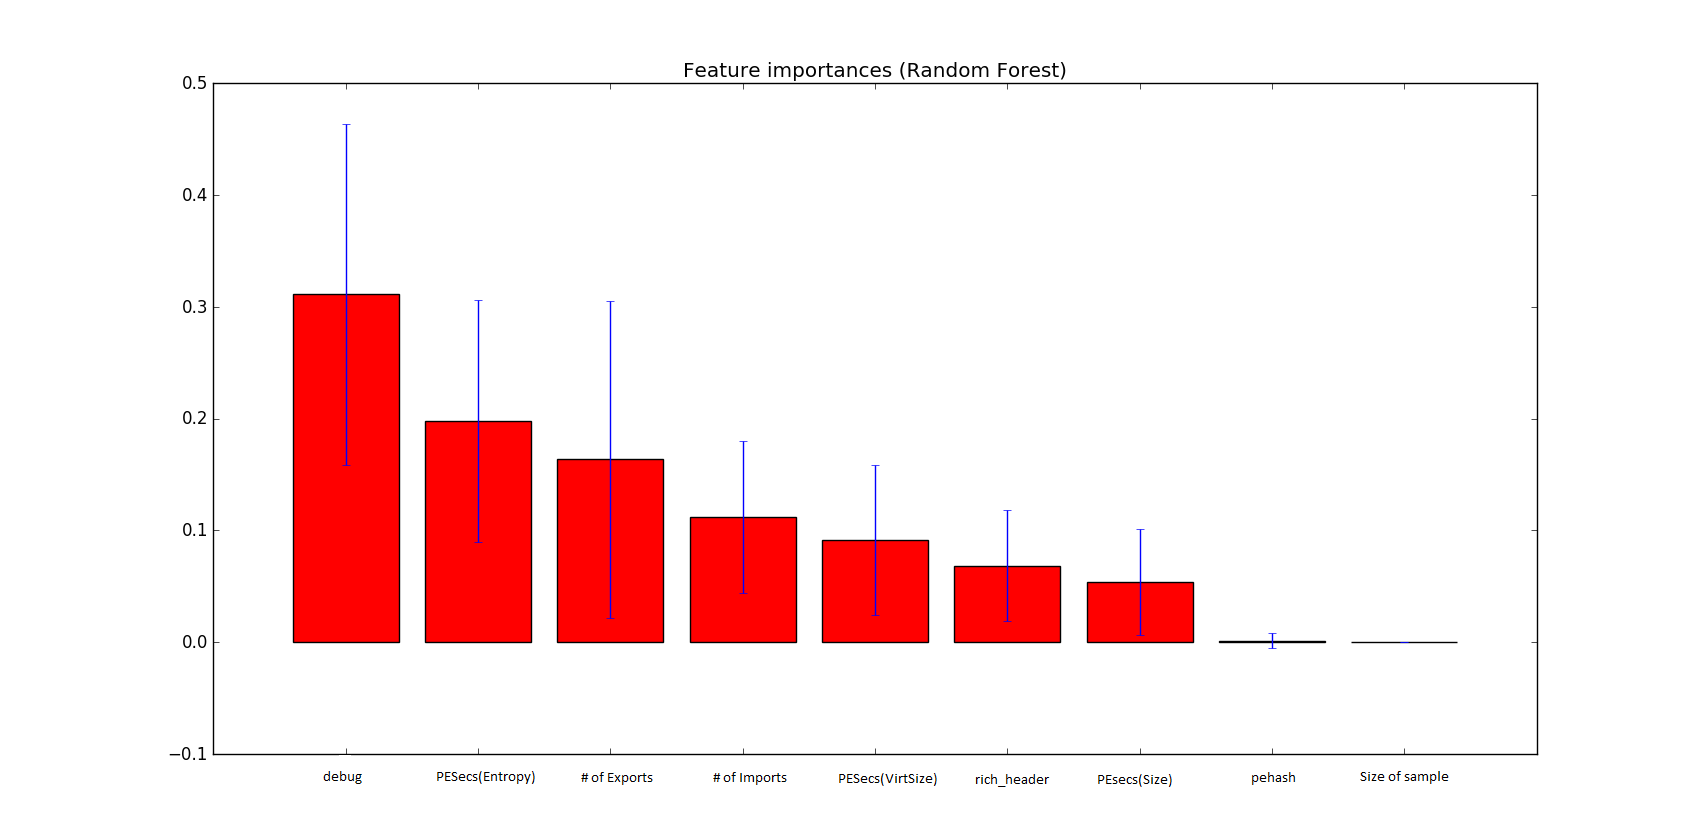
\includegraphics[width=6cm]{random_forest_feature_importances}
	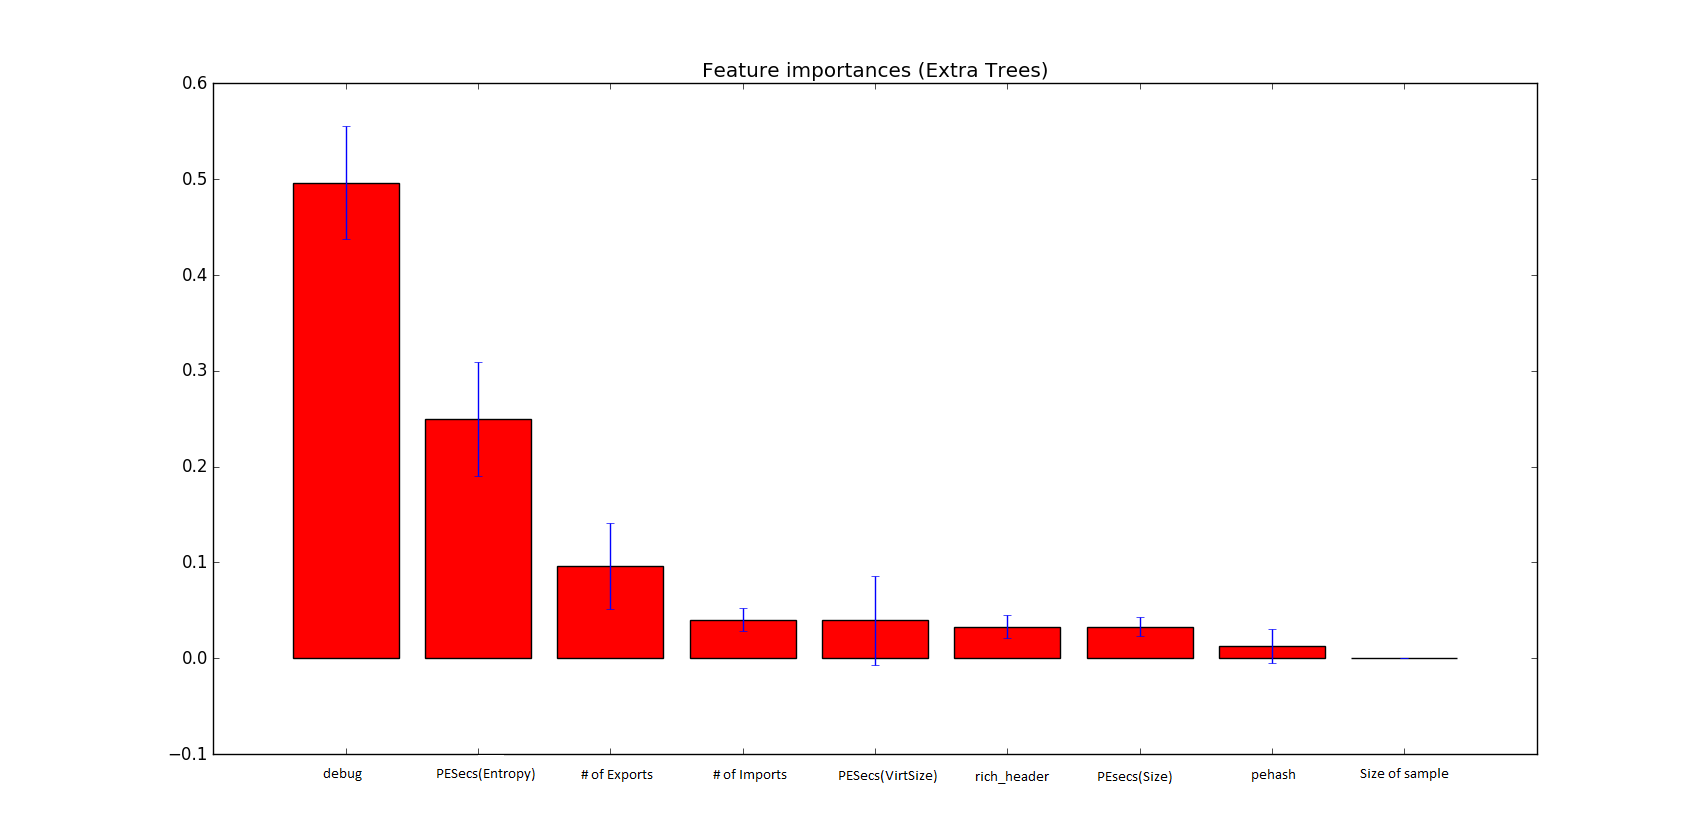
\includegraphics[width=6cm]{extra_trees_feature_importances}
	\centering
	\caption{Visualizing the relative importance of features using tree classifiers}
\end{figure}

\section{Results}
Results of the challenge are summarized in this section. We present results based upon training accuracies only. The results presented are achieved after feature scaling and random re-sampling and ten-fold cross validation. \\
Again, we report that Random Forest turned out to give the best accuracy. The authors tried their best to tune the Multi-Layer Perceptron to work, but could not quite achieve the accuracy of RF. One conclusion we can draw from the challenges so far is that Random Forest is an extremely robust and generic classifier that works really well in a lot of tasks. \\
We were also quite pleased with the overall accuracy achieved by our experiments. The features that we have extracted proved to be largely effective in distinguishing between the classes. Perhaps the subset of data provided to us was particularly easy to separate into these two classes, explaining the freakishly high accuracies achieved. \\\\\\\\
The optimal value of number of estimators for random forests is found to be: \textbf{93}\\
The optimal value of number of estimators for extra trees is found to be: \textbf{59}\\\\

\begin{table}[h]
	\centering
	\caption{Best Average Cross-Validation Accuracies}
	\begin{tabular}{ |p{5cm}||p{3cm}||p{3cm}|}
		\hline
		Technique                  &Cross Validation Accuracy & Testing Accuracy(Public Score)\\
		\hline
		Random Forest              								&97.242 &98.243\\
		Extra Trees													&96.33 & 97.901\\
		Multi Layer Perceptron(1 layer)	 			  		&92.75 &93.95\\
		Multi Layer Perceptron(3 layers)	 			  &93.67 &94.4\\
		Multi Layer Perceptron(4 layers)	 			  &93.66 &94.53\\
		Adaboost	 					            &96.221 &95.293\\
		KNN              				               &95.243 &92.998\\
		GradientBoostingClassifier	 						             &96.453 &85.439\\
		AdaBoostClassifier	 						             &95.838 &96.332\\
		DBScan	 						             &73.224 &Did Not Submit\\
		 \hline
	\end{tabular}
	\label{table}
\end{table}


%
% ---- Bibliography ----
%
\begin{thebibliography}{5}
%

\bibitem {hawkins:eke}
Hawkins D. , Basak S. , and Denise M. 
Assessing Model Fit by Cross-Validation
J. Chem. Inf. Comput. Sci., 2003, 43 (2), pp 579–586 (2003)

\end{thebibliography}
\end{document}
